
% Part 2 (Q3 OR - Q5)

\questionmarks{3}{a}{3} % OR
\textbf{રેડિયો રીસીવરની લાક્ષણિકતાઓ સમજાવો.}

\begin{solutionbox}
    \textbf{રેડિયો રીસીવરની લાક્ષણિકતાઓ:}

    \begin{center}
    \begin{tabulary}{\linewidth}{L L L}
        \hline
        \textbf{લાક્ષણિકતા} & \textbf{વ્યાખ્યા} & \textbf{મહત્વ} \\
        \hline
        \textbf{સંવેદનશીલતા} & નબળા સિગ્નલને એમ્પ્લિફાય કરવાની ક્ષમતા & મહત્તમ રિસેપ્શન રેન્જ નક્કી કરે છે \\
        \textbf{પસંદગીકારકતા} & આસપાસના સિગ્નલથી વાંછિત સિગ્નલને અલગ કરવાની ક્ષમતા & હસ્તક્ષેપ અટકાવે છે \\
        \textbf{વફાદારી} & મૂળ સિગ્નલને પુનઃ ઉત્પન્ન કરવામાં ચોકસાઈ & અવાજની ગુણવત્તા સુનિશ્ચિત કરે છે \\
        \textbf{છબી આવર્તન અસ્વીકૃતિ} & છબી આવર્તનને અસ્વીકાર કરવાની ક્ષમતા & ડુપ્લિકેટ રિસેપ્શન અટકાવે છે \\
        \hline
    \end{tabulary}
    \captionof{table}{રિસીવર લાક્ષણિકતાઓ}
    \end{center}

    \begin{center}
    \begin{tikzpicture}[
        mindmap, concept color=blue!20,
        every node/.style={concept, scale=0.8},
        grow cyclic,
        level 1/.style={level distance=3cm, sibling angle=90}
    ]
        \node [concept color=orange!40] {Receiver\\Characteristics}
        child { node {Sensitivity} }
        child { node {Selectivity} }
        child { node {Fidelity} }
        child { node {Image Rejection} };
    \end{tikzpicture}
    \captionof{figure}{મુખ્ય લાક્ષણિકતાઓ}
    \end{center}

    \begin{mnemonicbox}
    "SSFIM" - Select Signals Faithfully, Ignore Mirrors
    \end{mnemonicbox}
\end{solutionbox}

\questionmarks{3}{b}{4} % OR
\textbf{AM ડિટેક્ટર સર્કિટમાં થતા વિકૃતિઓના પ્રકારો સમજાવો.}

\begin{solutionbox}
    \textbf{AM ડિટેક્ટર સર્કિટમાં વિકૃતિઓના પ્રકારો:}

    \begin{center}
    \begin{tabulary}{\linewidth}{L L L}
        \hline
        \textbf{વિકૃતિ પ્રકાર} & \textbf{કારણ} & \textbf{નિવારણ} \\
        \hline
        \textbf{ડાયાગોનલ વિકૃતિ} & ખોટો સમય અચળાંક (RC બહુ મોટો) & યોગ્ય RC સમય અચળાંક \\
        \textbf{નકારાત્મક પીક ક્લિપિંગ} & ઉચ્ચ મોડ્યુલેશન ઇન્ડેક્સ + AC/DC લોડ મિસમેચ & યોગ્ય ડાયોડ બાયસિંગ / લોડ \\
        \textbf{હાર્મોનિક વિકૃતિ} & નોન-લીનિયર ડાયોડ લક્ષણો & ઉચ્ચ-ગુણવત્તાવાળા ડાયોડ \\
        \hline
    \end{tabulary}
    \captionof{table}{AM ડિટેક્ટર વિકૃતિઓ}
    \end{center}

    \textbf{વેવફોર્મ્સ:}

    \begin{center}
    \begin{tikzpicture}[xscale=2, yscale=1]
        % Normal
        \draw[gray, dotted] plot[domain=0:2*pi] (\x, {1 + 0.5*sin(deg(\x))});
        
        % Diagonal Clipping
        \begin{scope}[yshift=-2.5cm]
            \draw[->] (0,0) -- (6.5,0);
            \node[left] at (0,0.5) {Diagonal};
            \draw[thick, red] (0,1) -- (0.5,1.4) -- (1.5,0.8) -- (2.0,1.4); 
            \draw[blue] plot[domain=0:6] (\x, {1 + 0.5*sin(deg(\x))});
            \draw[red, thick] (1.6, 1.5) -- (2.5, 0.8); 
        \end{scope}

        % Negative Peak Clipping
        \begin{scope}[yshift=-5cm]
            \draw[->] (0,0) -- (6.5,0);
            \node[left] at (0,0.5) {Negative Peak};
            \draw[blue] plot[domain=0:6] (\x, {1 + 0.8*sin(deg(\x))});
            \draw[red, thick] (3.5, 0) -- (5.5, 0); 
        \end{scope}
    \end{tikzpicture}
    \captionof{figure}{વિકૃતિ પ્રકારો}
    \end{center}

    \begin{mnemonicbox}
    "DNHF" - Diagonal Negative Harmonics Frequency
    \end{mnemonicbox}
\end{solutionbox}

\questionmarks{3}{c}{7} % OR
\textbf{સુપરહીટેરોડીન AM રીસીવરનો બ્લોક ડાયાગ્રામ દોરો અને તેને સમજાવો.}

\begin{solutionbox}
    \textbf{સુપરહીટેરોડીન AM રીસીવર:}

    \begin{center}
    \begin{tikzpicture}[auto, node distance=1.5cm,
        block/.style={draw, rectangle, minimum height=3em, minimum width=3.5em, align=center},
        >=stealth
    ]
        \node [coordinate] (ant) {};
        \node [block, right=0.5cm of ant] (rf) {RF Amp};
        \node [block, right=1cm of rf] (mix) {Mixer};
        \node [block, below=1cm of mix] (lo) {Local Osc};
        \node [block, right=1cm of mix] (if) {IF Amp};
        \node [block, right=1cm of if] (det) {Detector};
        \node [block, right=1cm of det] (af) {AF Amp};
        \node [coordinate, right=0.5cm of af] (spk) {};
        \node [block, above=1cm of if] (agc) {AGC};

        \draw [->] (ant) -- node[above]{Antenna} (rf);
        \draw [->] (rf) -- (mix);
        \draw [->] (lo) -- (mix);
        \draw [->] (mix) -- node[above]{IF} (if);
        \draw [->] (if) -- (det);
        \draw [->] (det) -- (af);
        \draw [->] (af) -- node[right]{Speaker} (spk);
        
        \draw [->] (det.north) |- (agc.east);
        \draw [->] (agc.west) -| (rf.north);
        \draw [->] (agc.south) -- (if.north);

    \end{tikzpicture}
    \captionof{figure}{સુપરહીટેરોડીન રીસીવર}
    \end{center}

    \textbf{દરેક બ્લોકનું કાર્ય:}
    \begin{itemize}
        \item \textbf{RF એમ્પ્લિફાયર}: નબળા RF સિગ્નલને એમ્પ્લિફાય કરે છે, જે સંવેદનશીલતા અને પસંદગીકારકતા સુધારે છે.
        \item \textbf{મિક્સર}: RF ($f_s$) અને LO ($f_o$) ને મિક્સ કરીને IF ($f_o - f_s$) ઉત્પન્ન કરે છે.
        \item \textbf{લોકલ ઓસીલેટર}: આવતા સિગ્નલથી નિશ્ચિત આવર્તન પર સિગ્નલ ઉત્પન્ન કરે છે.
        \item \textbf{IF એમ્પ્લિફાયર}: નિશ્ચિત મધ્યવર્તી આવર્તન (455 kHz) પર એમ્પ્લિફિકેશન પૂરું પાડે છે.
        \item \textbf{ડિટેક્ટર}: મોડ્યુલેટેડ સિગ્નલમાંથી ઓડિયો એક્સ્ટ્રેક્ટ કરે છે.
        \item \textbf{AF એમ્પ્લિફાયર}: સ્પીકર ચલાવવા માટે ઓડિયોને એમ્પ્લિફાય કરે છે.
        \item \textbf{AGC}: રિસીવરના આઉટપુટ લેવલને સ્થિર રાખે છે.
    \end{itemize}

    \begin{mnemonicbox}
    "RMLIDAS" - Radio Mixing Local Intermediate Detected Audio Signals
    \end{mnemonicbox}
\end{solutionbox}

\questionmarks{4}{a}{3}
\textbf{એનાલોગથી ડિજિટલ રૂપાંતરણમાં વપરાતી ક્વોન્ટાઇઝેશનની પ્રક્રિયા સમજાવો.}

\begin{solutionbox}
    \textbf{ક્વોન્ટાઇઝેશન પ્રક્રિયા:}
    \begin{enumerate}
        \item \textbf{સેમ્પલિંગ}: સમયને અસતત (discretize) બનાવવો.
        \item \textbf{લેવલ ફાળવણી}: એમ્પ્લિટ્યુડ રેન્જને $L$ ડિસ્ક્રીટ લેવલમાં વિભાજિત કરવી.
        \item \textbf{અસાઇનમેન્ટ}: દરેક સેમ્પલ વેલ્યુને નજીકના લેવલમાં મેપ કરવી.
        \item \textbf{એનકોડિંગ}: લેવલ ઇન્ડેક્સને બાઇનરીમાં રૂપાંતરિત કરવું.
    \end{enumerate}

    \begin{center}
    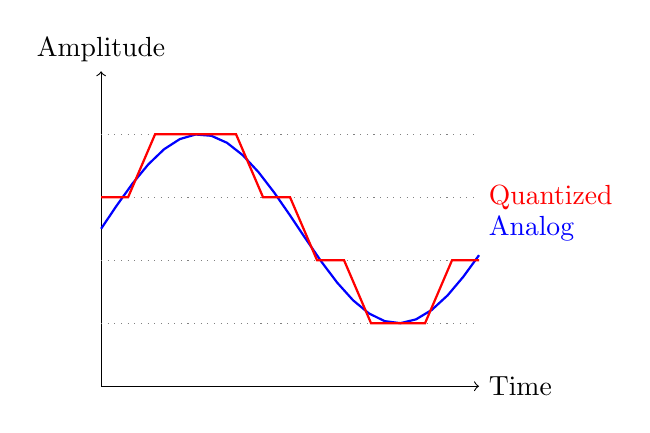
\begin{tikzpicture}[scale=0.8]
        \draw[->] (0,0) -- (6,0) node[right]{Time};
        \draw[->] (0,0) -- (0,5) node[above]{Amplitude};
        
        \foreach \y in {1,2,3,4} \draw[gray, dotted] (0,\y) -- (6,\y);
        
        \draw[blue, thick] plot[domain=0:6] (\x, {2.5 + 1.5*sin(deg(\x))});
        \draw[red, thick, step=0.5] plot[domain=0:6, samples=15] (\x, {round(2.5 + 1.5*sin(deg(\x)))});
        
        \node[right, blue] at (6, 2.5) {Analog};
        \node[right, red] at (6, 3) {Quantized};
    \end{tikzpicture}
    \captionof{figure}{ક્વોન્ટાઇઝેશન સ્ટેરકેસ}
    \end{center}

    \begin{mnemonicbox}
    "SLAB" - Sample Levels Assign Binary
    \end{mnemonicbox}
\end{solutionbox}

\questionmarks{4}{b}{4}
\textbf{સેમ્પલિંગ તકનીકોની સરખામણી આપો.}

\begin{solutionbox}
    \textbf{સેમ્પલિંગ તકનીકોની સરખામણી:}

    \begin{center}
    \begin{tabulary}{\linewidth}{L L L}
        \hline
        \textbf{તકનીક} & \textbf{વર્ણન} & \textbf{ફાયદા/ગેરલાભ} \\
        \hline
        Ideal & ત્વરિત આવેગ & માત્ર સૈદ્ધાંતિક \\
        Natural & પલ્સ ટોપ સિગ્નલના આકારને અનુસરે છે & જટિલ જનરેશન \\
        Flat-top & પલ્સ ટોપ ફ્લેટ છે (સેમ્પલ અને હોલ્ડ) & જનરેટ કરવા માટે સરળ / એપર્ચર એરર \\
        \hline
    \end{tabulary}
    \captionof{table}{સેમ્પલિંગ પ્રકારો}
    \end{center}

    \begin{center}
    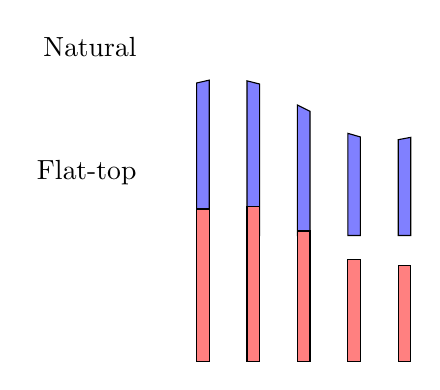
\begin{tikzpicture}[scale=0.8]
        \node[left] at (0,3) {Natural};
        \foreach \x in {1,2,3,4,5} {
             \draw[fill=blue!50] (0.8*\x, 0) -- (0.8*\x, {2+0.5*sin(deg(\x))}) -- (0.8*\x+0.2, {2+0.5*sin(deg(\x+0.2))}) -- (0.8*\x+0.2, 0) -- cycle;
        }

        \node[left] at (0,1) {Flat-top};
        \foreach \x in {1,2,3,4,5} {
             \draw[fill=red!50] (0.8*\x, -2) rectangle (0.8*\x+0.2, {0.5*sin(deg(\x))});
        }
    \end{tikzpicture}
    \captionof{figure}{નેચરલ વિરુદ્ધ ફ્લેટ-ટોપ સેમ્પલિંગ}
    \end{center}

    \begin{mnemonicbox}
    "INF" - Ideal Natural Flat
    \end{mnemonicbox}
\end{solutionbox}

\questionmarks{4}{c}{7}
\textbf{PCM ટ્રાન્સમીટર અને રીસીવરનો બ્લોક ડાયાગ્રામ દોરો અને સમજાવો.}

\begin{solutionbox}
    \textbf{Pulse Code Modulation (PCM):}

    \textbf{ટ્રાન્સમીટર:}
    \begin{center}
    \begin{tikzpicture}[auto, node distance=1.2cm,
        block/.style={draw, rectangle, minimum height=2.5em, text width=4em, align=center},
        >=stealth
    ]
        \node[coordinate](in){};
        \node[block, right=0.5cm of in](lpf){LPF};
        \node[block, right=0.8cm of lpf](sh){S/H};
        \node[block, right=0.8cm of sh](q){Quantizer};
        \node[block, right=0.8cm of q](enc){Encoder};
        \node[block, right=0.8cm of enc](p2s){P/S};
        \node[coordinate, right=0.5cm of p2s](out){};

        \draw[->] (in) -- (lpf);
        \draw[->] (lpf) -- (sh);
        \draw[->] (sh) -- (q);
        \draw[->] (q) -- (enc);
        \draw[->] (enc) -- (p2s);
        \draw[->] (p2s) -- node[above]{PCM Out} (out);
    \end{tikzpicture}
    \end{center}

    \textbf{રિસીવર:}
    \begin{center}
    \begin{tikzpicture}[auto, node distance=1.2cm,
        block/.style={draw, rectangle, minimum height=2.5em, text width=4em, align=center},
        >=stealth
    ]
        \node[coordinate](in){};
        \node[block, right=0.5cm of in](regen){Regeneration\\Circuit};
        \node[block, right=0.8cm of regen](dec){Decoder};
        \node[block, right=0.8cm of dec](recon){Reconstruction\\Filter};
        \node[coordinate, right=0.5cm of recon](out){};

        \draw[->] (in) -- node[above]{PCM In} (regen);
        \draw[->] (regen) -- (dec);
        \draw[->] (dec) -- (recon);
        \draw[->] (recon) -- node[above]{Analog Out} (out);
    \end{tikzpicture}
    \end{center}

    \begin{mnemonicbox}
    "FSQEMT" - Filter, Sample, Quantize, Encode, Multiplex, Transmit
    \end{mnemonicbox}
\end{solutionbox}

\questionmarks{4}{a}{3} % OR
\textbf{Nyquist પ્રમેય જણાવો અને સમજાવો.}

\begin{solutionbox}
    \textbf{Nyquist સેમ્પલિંગ પ્રમેય:}
    
    બેન્ડ-લિમિટેડ સિગ્નલને સંપૂર્ણ રીતે પુનઃનિર્માણ કરવા માટે, સેમ્પલિંગ આવર્તન $f_s$ સિગ્નલમાં હાજર મહત્તમ આવર્તન ઘટક $f_{max}$ ના ઓછામાં ઓછા બમણા હોવા જોઈએ.
    \[ f_s \ge 2 f_{max} \]
    
    \begin{itemize}
        \item $2f_{max}$ ને \textbf{Nyquist Rate} કહેવાય છે.
        \item જો $f_s < 2f_{max}$, તો \textbf{Aliasing} થાય છે (સ્પેક્ટ્રલ ઘટકોનું ઓવરલેપિંગ).
    \end{itemize}

    \begin{center}
    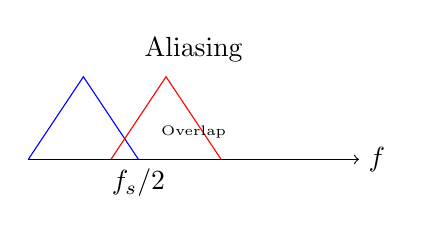
\begin{tikzpicture}[scale=0.7]
        % Aliasing
        \draw[->] (0,0) -- (6,0) node[right]{$f$};
        \node at (3,2) {Aliasing};
        \draw[blue] (0,0) -- (1,1.5) -- (2,0);
        \draw[red] (1.5,0) -- (2.5,1.5) -- (3.5,0);
        \node[below] at (2,0) {$f_s/2$};
        \node[font=\tiny] at (3,0.5) {Overlap};
    \end{tikzpicture}
    \captionof{figure}{અન્ડરસેમ્પલિંગની અસર (એલિયાસિંગ)}
    \end{center}

    \begin{mnemonicbox}
    "DMFSA" - Double Maximum Frequency Stops Aliasing
    \end{mnemonicbox}
\end{solutionbox}

\questionmarks{4}{b}{4} % OR
\textbf{DM, ADM અને DPCMની સરખામણી આપો.}

\begin{solutionbox}
    \textbf{સરખામણી:}

    \begin{center}
    \begin{tabulary}{\linewidth}{L L L L}
        \hline
        \textbf{લક્ષણ} & \textbf{Delta Mod (DM)} & \textbf{Adaptive DM} & \textbf{DPCM} \\
        \hline
        \textbf{આધાર} & 1 Bit તફાવત & ચલ સ્ટેપ સાઇઝ & Multi-bit તફાવત \\
        \textbf{સ્ટેપ સાઇઝ} & સ્થિર (Fixed) & ચલ (Variable) & સ્થિર/એડેપ્ટિવ \\
        \textbf{કોડિંગ} & 1 Bit/sample & 1 Bit/sample & $>1$ Bit/sample \\
        \textbf{ભૂલો} & સ્લોપ ઓવરલોડ, ગ્રેન્યુલર & ઓછી ભૂલો & ક્વોન્ટાઇઝેશન નોઇઝ \\
        \textbf{જટિલતા} & સૌથી ઓછી & મધ્યમ & વધુ \\
        \hline
    \end{tabulary}
    \captionof{table}{DM vs ADM vs DPCM}
    \end{center}

    \begin{mnemonicbox}
    "SAMD" - Single-bit, Adaptive-bit, Multi-bit Difference
    \end{mnemonicbox}
\end{solutionbox}

\questionmarks{4}{c}{7} % OR
\textbf{ડિફરન્શિયલ PCM (DPCM) ટ્રાન્સમીટર અને રીસીવરની કાર્યગીરી સમજાવો.}

\begin{solutionbox}
    \textbf{DPCM સિદ્ધાંત:}
    ચોક્કસ સેમ્પલ વેલ્યુને બદલે, આ અગાઉના સેમ્પલના આધારે આગાહી કરેલ મૂલ્ય અને વર્તમાન સેમ્પલ વચ્ચેના \textit{તફાવત}ને એનકોડ કરે છે.

    \textbf{DPCM ટ્રાન્સમીટર:}
    \begin{center}
    \begin{tikzpicture}[auto, node distance=1.5cm, >=stealth]
        \node[draw, rectangle, minimum height=2em] (quant) {Quantizer};
        \node[draw, rectangle, minimum height=2em, right=1cm of quant] (enc) {Encoder};
        \node[right=1cm of enc] (out) {};
        
        \node[draw, circle, left=1cm of quant] (sub) {$\Sigma$};
        \node[left=1cm of sub] (in) {};
        
        \node[draw, circle, below=1cm of quant] (add) {$\Sigma$};
        \node[draw, rectangle, minimum height=2em, left=1cm of add] (pred) {Predictor};
        
        \draw[->] (in) -- (sub);
        \draw[->] (sub) -- node[above]{\footnotesize E} (quant);
        \draw[->] (quant) -- (enc);
        \draw[->] (enc) -- (out);
        
        \draw[->] (quant) -- (add);
        \draw[->] (add) -- (pred);
        \draw[->] (pred) -| (sub);
        \draw[->] (pred) -- (add);
    \end{tikzpicture}
    \captionof{figure}{DPCM ટ્રાન્સમીટર}
    \end{center}

    \textbf{DPCM રિસીવર:}
    \begin{center}
    \begin{tikzpicture}[auto, node distance=1.5cm,
        block/.style={draw, rectangle, minimum height=2.5em, text width=4em, align=center},
        sum/.style={draw, circle, inner sep=0pt, minimum size=6mm},
        >=stealth
    ]
        \node[block](dec){Decoder};
        \node[sum, right=0.8cm of dec](sum){+};
        \node[block, below=1cm of sum](pred){Predictor};
        \node[block, right=0.8cm of sum](lpf){LPF};
        
        \draw[->] (dec) -- (sum);
        \draw[->] (sum) -- (lpf);
        \draw[->] (sum.east) |- (pred.east);
        \draw[->] (pred) -| (sum.south);
    \end{tikzpicture}
    \captionof{figure}{DPCM રિસીવર}
    \end{center}

    \begin{mnemonicbox}
    "PSQD" - Predict Subtract Quantize Difference
    \end{mnemonicbox}
\end{solutionbox}

\questionmarks{5}{a}{3}
\textbf{TDMA ફ્રેમનું વર્ણન કરો.}

\begin{solutionbox}
    \textbf{TDMA ફ્રેમ સ્ટ્રક્ચર:}

    ટાઇમ ડિવિઝન મલ્ટિપલ એક્સેસ બહુવિધ વપરાશકર્તાઓને અલગ ટાઇમ સ્લોટ્સ ફાળવીને સમાન આવર્તન શેર કરવાની મંજૂરી આપે છે.

    \begin{center}
    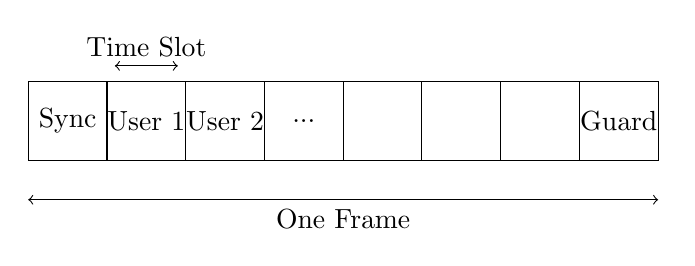
\begin{tikzpicture}
        \draw (0,0) rectangle (8,1);
        \foreach \x in {1,2,3,4,5,6,7} \draw (\x,0) -- (\x,1);
        \node at (0.5,0.5) {Sync};
        \node at (1.5,0.5) {User 1};
        \node at (2.5,0.5) {User 2};
        \node at (3.5,0.5) {...};
        \node at (7.5,0.5) {Guard};
        
        \draw[<->] (0, -0.5) -- (8,-0.5) node[midway, below] {One Frame};
        \draw[<->] (1.1, 1.2) -- (1.9, 1.2) node[midway, above] {Time Slot};
    \end{tikzpicture}
    \captionof{figure}{TDMA ફ્રેમ}
    \end{center}

    ઘટકો: પ્રીએમ્બલ (Sync), માહિતી સંદેશ, ગાર્ડ બિટ્સ (ગેપ).

    \begin{mnemonicbox}
    "SITDA" - Slots In Time Divide Access
    \end{mnemonicbox}
\end{solutionbox}

\questionmarks{5}{b}{4}
\textbf{4 સ્તરના ડિજિટલ મલ્ટિપ્લેક્સિંગ વંશવેલો દોરો અને સમજાવો.}

\begin{solutionbox}
    \textbf{ડિજિટલ મલ્ટિપ્લેક્સિંગ હાયરાર્કી (North American T-carrier):}

    \begin{center}
    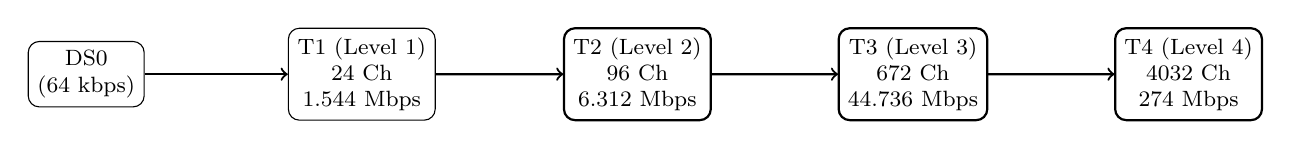
\begin{tikzpicture}[
        grow=right,
        level 1/.style={level distance=3.5cm, sibling distance=2cm},
        level 2/.style={level distance=3.5cm, sibling distance=1.5cm},
        edge from parent/.style={draw, ->, thick},
        every node/.style={draw, rectangle, rounded corners, align=center, font=\footnotesize}
    ]
        \node {DS0\\(64 kbps)}
            child {
                node {T1 (Level 1)\\24 Ch\\1.544 Mbps}
                child {
                    node {T2 (Level 2)\\96 Ch\\6.312 Mbps}
                    child {
                        node {T3 (Level 3)\\672 Ch\\44.736 Mbps}
                        child {
                            node {T4 (Level 4)\\4032 Ch\\274 Mbps}
                        }
                    }
                }
            };
    \end{tikzpicture}
    \captionof{figure}{T-Carrier હાયરાર્કી}
    \end{center}

    \begin{mnemonicbox}
    "PSTQ" - Primary, Secondary, Tertiary, Quaternary Levels
    \end{mnemonicbox}
\end{solutionbox}

\questionmarks{5}{c}{7}
\textbf{PCM-TDM સિસ્ટમનો બ્લોક ડાયાગ્રામ દોરો અને સમજાવો.}

\begin{solutionbox}
    \textbf{PCM-TDM બ્લોક ડાયાગ્રામ:}

    \begin{center}
    \begin{tikzpicture}[auto, node distance=1.2cm,
        block/.style={draw, rectangle, minimum height=2.5em, text width=4em, align=center},
        >=stealth
    ]
        % Inputs
        \node (in1) {Ch 1};
        \node [below=0.6cm of in1] (in2) {Ch 2};
        \node [below=0.6cm of in2] (in3) {Ch 3};
        
        % LPFs
        \node [block, right=0.5cm of in1] (lpf1) {LPF};
        \node [block, right=0.5cm of in2] (lpf2) {LPF};
        \node [block, right=0.5cm of in3] (lpf3) {LPF};
        
        % Commutator (Sampler/MUX)
        \node [draw, circle, right=1cm of lpf2, minimum size=1cm] (mux) {MUX};
        
        % PCM Blocks
        \node [block, right=1cm of mux] (pcm) {PCM Encoder};
        \node [coordinate, right=0.5cm of pcm] (tx) {};
        
        % Rx side
        \node [block, right=1.5cm of pcm] (dec) {PCM Decoder};
        \node [draw, circle, right=1cm of dec, minimum size=1cm] (demux) {DeMUX};
        \node [block, right=1cm of demux] (lpf_out) {LPFs};
        
        \draw[->] (in1) -- (lpf1);
        \draw[->] (in2) -- (lpf2);
        \draw[->] (in3) -- (lpf3);
        
        \draw[->] (lpf1) -- (mux);
        \draw[->] (lpf2) -- (mux);
        \draw[->] (lpf3) -- (mux);
        
        \draw[->] (mux) -- (pcm);
        \draw[dashed, ->] (pcm) -- node[above]{TDM Link} (dec);
        
        \draw[->] (dec) -- (demux);
        \draw[->] (demux) -- (lpf_out);
        
    \end{tikzpicture}
    \captionof{figure}{PCM-TDM સિસ્ટમ}
    \end{center}

    **પ્રક્રિયા**:
    \begin{enumerate}
        \item બહુવિધ એનાલોગ ચેનલો LPF દ્વારા બેન્ડ-લિમિટેડ હોય છે.
        \item કોમ્યુટેટર દરેક ચેનલને ક્રમિક રીતે સેમ્પલ કરે છે (AM-TDM).
        \item સંયુક્ત TDM સિગ્નલ એક PCM એનકોડરમાં પ્રવેશે છે.
        \item કોડેડ બિટ્સ ઇન્ટરલેસ્ડ ટ્રાન્સમિટ થાય છે.
    \end{enumerate}

    \begin{mnemonicbox}
    "MACSDL" - Many Analog Channels Share Digital Link
    \end{mnemonicbox}
\end{solutionbox}

\questionmarks{5}{a}{3} % OR
\textbf{ડિજિટલ કમ્યુનિકેશનના ફાયદા અને ગેરફાયદાની સૂચિ બનાવો.}

\begin{solutionbox}
    \textbf{ફાયદા અને ગેરફાયદા:}

    \begin{center}
    \begin{tabulary}{\linewidth}{L L}
        \hline
        \textbf{ફાયદા} & \textbf{ગેરફાયદા} \\
        \hline
        ઉત્તમ નોઇઝ ઇમ્યુનિટી & વધારે બેન્ડવિડ્થની જરૂર \\
        એરર ડિટેક્શન અને કરેક્શન & સિસ્ટમની જટિલતા \\
        સરળ મલ્ટિપ્લેક્સિંગ (TDM) & સિન્ક્રોનાઇઝેશનની જરૂર \\
        સુરક્ષિત (એન્ક્રિપ્શન) & ક્વોન્ટાઇઝેશન નોઇઝ \\
        \hline
    \end{tabulary}
    \captionof{table}{ડિજિટલ કોમ્યુનિકેશન ફાયદા/ગેરફાયદા}
    \end{center}

    \begin{mnemonicbox}
    "NEMBB" - Noise-resistant, Error-correcting, Multiplex-friendly But Bandwidth-hungry
    \end{mnemonicbox}
\end{solutionbox}

\questionmarks{5}{b}{4} % OR
\textbf{ચેનલ કોડિંગ તકનીકોની સૂચિ બનાવો, તેમાંથી કોઇ પણ એકને ઉદાહરણ સાથે સમજાવો.}

\begin{solutionbox}
    \textbf{ચેનલ કોડિંગ તકનીકો:}
    \begin{itemize}
        \item Linear Block Codes (દા.ત., Hamming)
        \item Cyclic Codes (દા.ત., CRC)
        \item Convolutional Codes
        \item Turbo Codes
    \end{itemize}

    \textbf{ઉદાહરણ: Hamming Code (7,4)}
    \begin{itemize}
        \item 4 ડેટા બિટ્સ લે છે, 3 પેરિટી બિટ્સ ઉમેરે છે ($n=7, k=4$).
        \item 1 બિટ એરર સુધારી શકે છે.
        \item પેરિટી બિટ્સ $2^0, 2^1, 2^2...$ પોઝિશન પર મૂકવામાં આવે છે.
        \item જો Data = 1010, Encoded = $p_1 p_2 1 p_4 0 1 0$. ચોક્કસ પોઝિશનના XOR પર આધારિત પેરિટી ગણતરી.
    \end{itemize}

    \begin{mnemonicbox}
    "PBPDB" - Parity Bits Protect Data Bits
    \end{mnemonicbox}
\end{solutionbox}

\questionmarks{5}{c}{7} % OR
\textbf{મૂળભૂત ટાઇમ ડોમેન ડિજિટલ મલ્ટિપ્લેક્સિંગની ચર્ચા કરો. TDM સિસ્ટમના ફાયદા અને ગેરફાયદા જણાવો.}

\begin{solutionbox}
    \textbf{ટાઇમ ડિવિઝન મલ્ટિપલ એક્સેસ (TDM):}
    એવી તકનીક જ્યાં બહુવિધ અલગ સિગ્નલો એક ચેનલ પર સમયના ડોમેનમાં ઇન્ટરલીવ કરીને ટ્રાન્સમિટ થાય છે.

    \textbf{ફાયદા:}
    \begin{itemize}
        \item એક સમયે એક વપરાશકર્તા દ્વારા સંપૂર્ણ બેન્ડવિડ્થનો ઉપયોગ થાય છે.
        \item લવચીક સિગ્નલ હેન્ડલિંગ (ડિજિટલ).
        \item FDM ની સરખામણીમાં સરળ સર્કિટરી.
    \end{itemize}

    \textbf{ગેરફાયદા:}
    \begin{itemize}
        \item કડક સિન્ક્રોનાઇઝેશનની જરૂર છે.
        \item જો સ્લોટ્સ ખાલી હોય તો બેન્ડવિડ્થનો બગાડ.
        \item મલ્ટિપાથ ડિસ્ટોર્શન TDM ને FDM કરતા વધુ અસર કરે છે.
    \end{itemize}

    \begin{center}
    \begin{tikzpicture}[auto, node distance=1cm, >=stealth]
        \node (s1) {S1};
        \node [below=0.5cm of s1] (s2) {S2};
        \node [draw, rectangle, right=1cm of s1] (mux) {MUX};
        \node [right=2cm of mux] (dmux) {DeMUX};
        
        \draw[->] (s1) -- (mux);
        \draw[->] (s2) -- (mux);
        \draw[->] (mux) -- (dmux);
    \end{tikzpicture}
    \captionof{figure}{મૂળભૂત TDM}
    \end{center}

    \begin{mnemonicbox}
    "TSSBSR" - Time Slots Shared But Sync Required
    \end{mnemonicbox}
\end{solutionbox}

\end{document}
